\documentclass[10pt,pdf,utf8,aspectratio=169,xcolor=dvipsnames,x11names,center]{beamer}

\usepackage[T2A]{fontenc}
\usepackage[english,russian]{babel}
\usepackage[utf8]{inputenc}

\usepackage{pgfpages}
%%\setbeameroption{show notes}
%%\setbeameroption{show notes on second screen=right}

\usepackage{dirtytalk}

\usepackage{listings}

\definecolor{light-gray}{gray}{0.95}
\lstset{
language=Python,                             % Code langugage
basicstyle=\small,                   % Code font, Examples: \footnotesize, \ttfamily
keywordstyle=\color{JungleGreen},        % Keywords font ('*' = uppercase)
commentstyle=\color{gray},              % Comments font
numbers=left,                           % Line nums position
numberstyle=\tiny,                      % Line-numbers fonts
stringstyle=\color{BrickRed},          %
stepnumber=1,                           % Step between two line-numbers
numbersep=5pt,                          % How far are line-numbers from code
backgroundcolor=\color{light-gray},     % Choose background color
frame=lines,                            % A frame around the code
tabsize=4,                              % Default tab size
captionpos=b,                           % Caption-position = bottom
breaklines=true,                        % Automatic line breaking?
breakatwhitespace=false,                % Automatic breaks only at whitespace?
showspaces=false,                       % Don't make spaces visible
showstringspaces=false,                 % Don't show spaces in string literals 
showtabs=false,                         % Don't make tabs visible
}

\title{Minsk Python Meetup 2018→}

\author[]{stas@garage22.net}

\date{Minsk Python Meetup\\November 2018}

\begin{document}

\begin{frame}
  \begin{figure}
    
\includegraphics[scale=0.88]{Slides-01-title}
  \end{figure}
\end{frame}

\begin{frame}
  \begin{figure}
    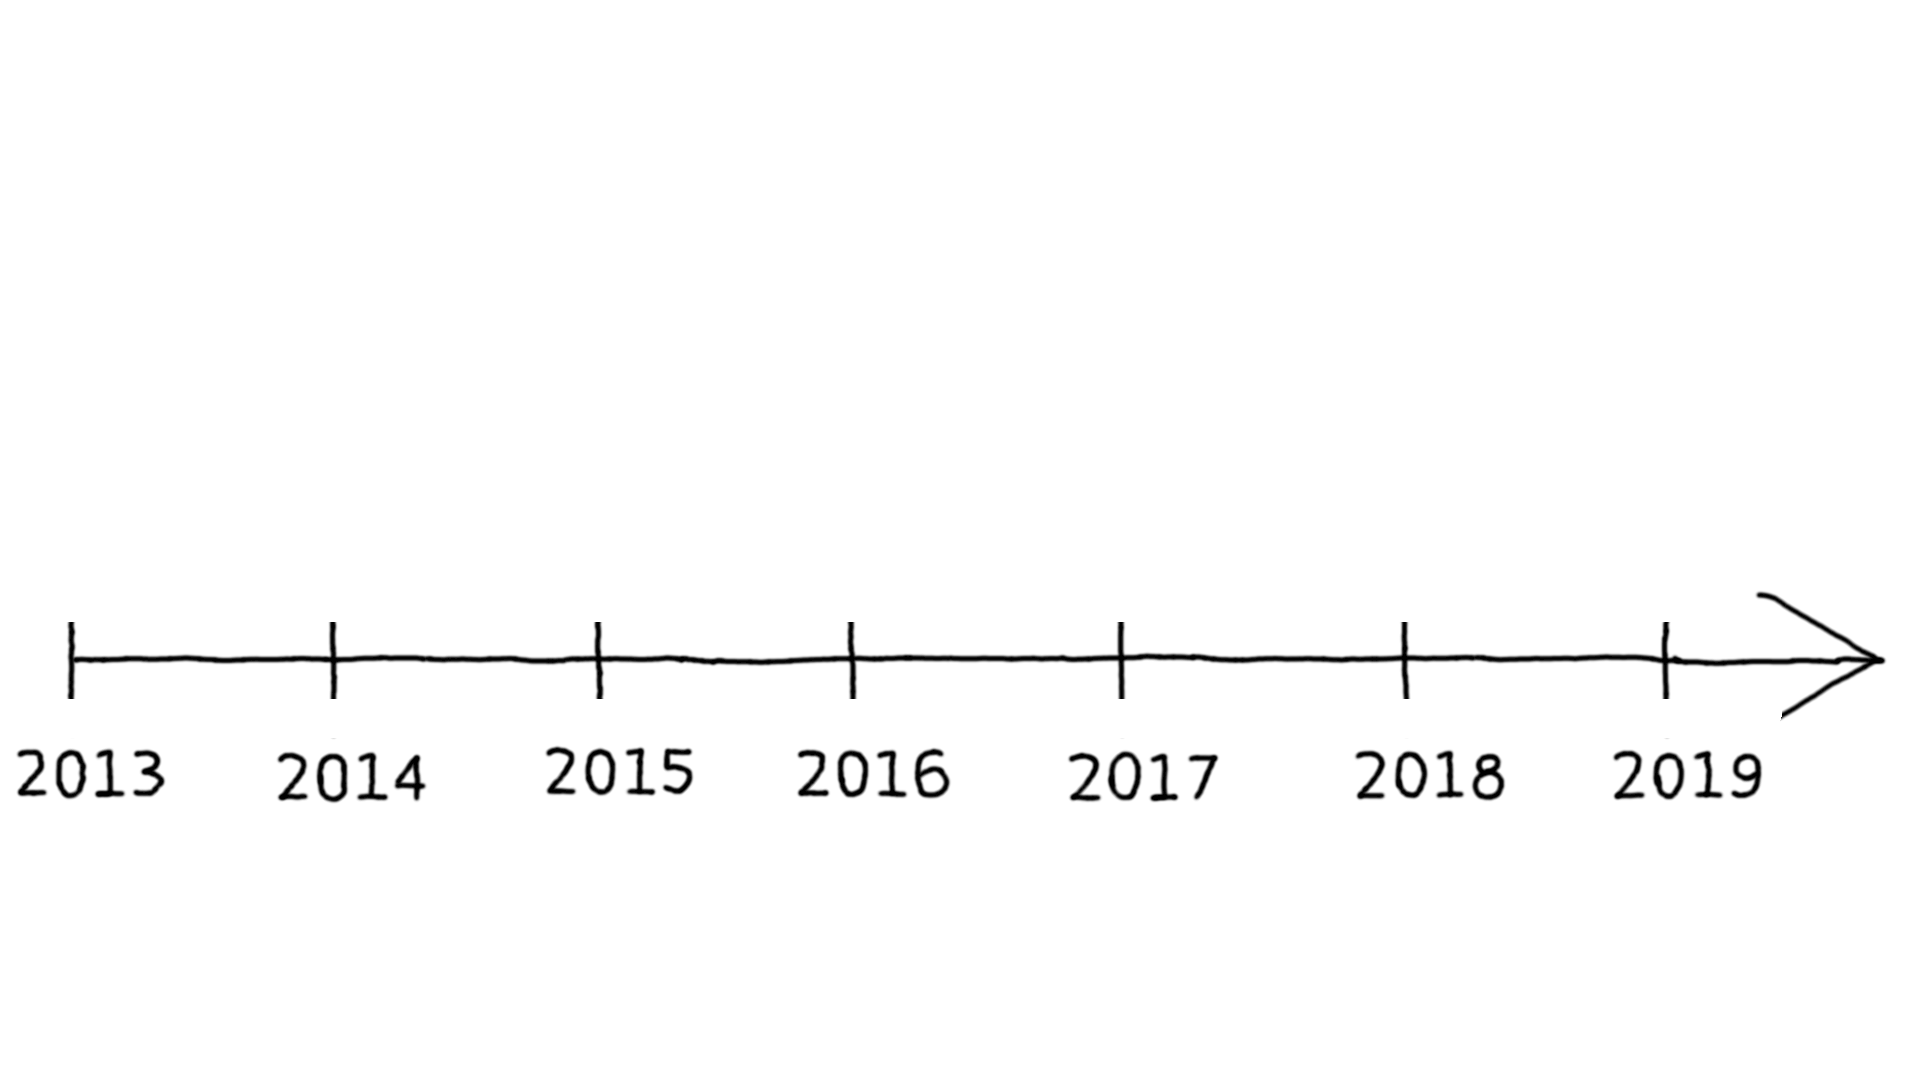
\includegraphics[scale=0.88]{Slides-02-01}
  \end{figure}
\end{frame}

\begin{frame}
  \begin{figure}
    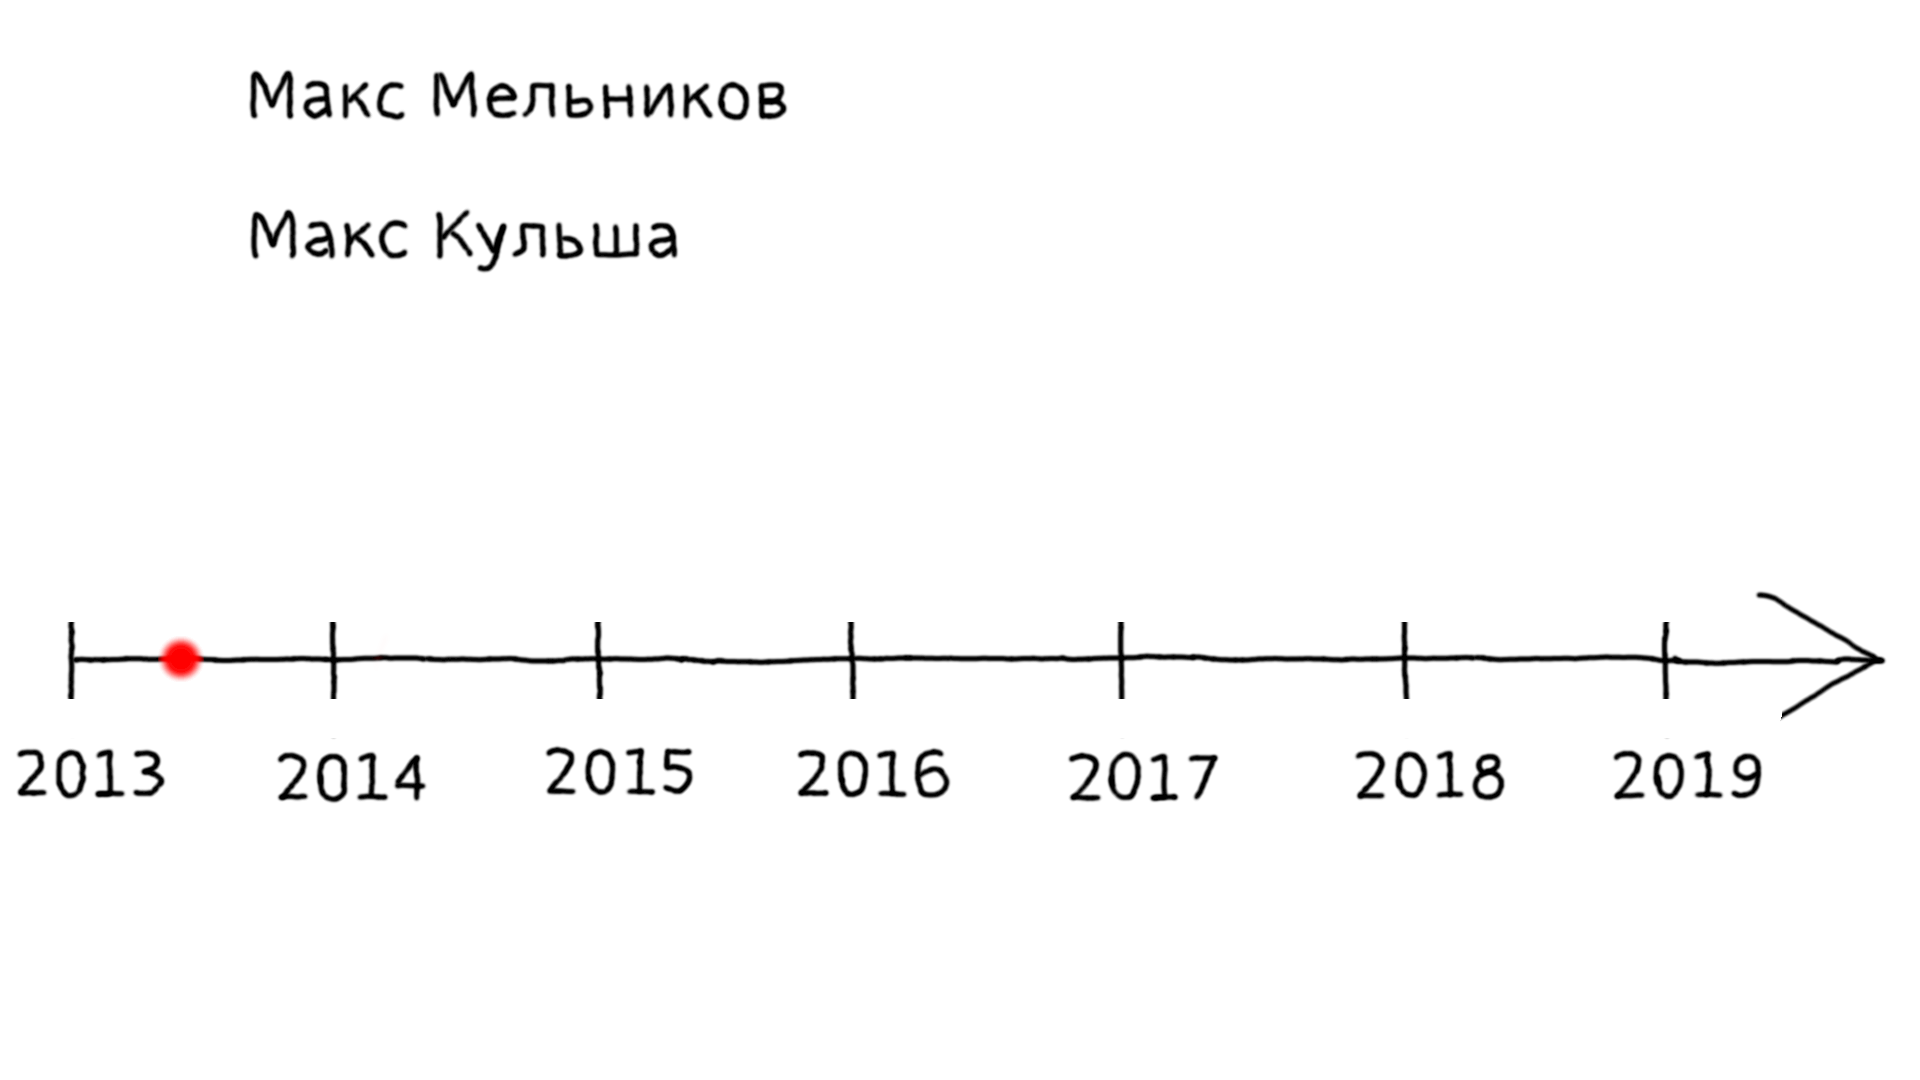
\includegraphics[scale=0.88]{Slides-02-02}
  \end{figure}
\end{frame}

\begin{frame}
  \begin{figure}
    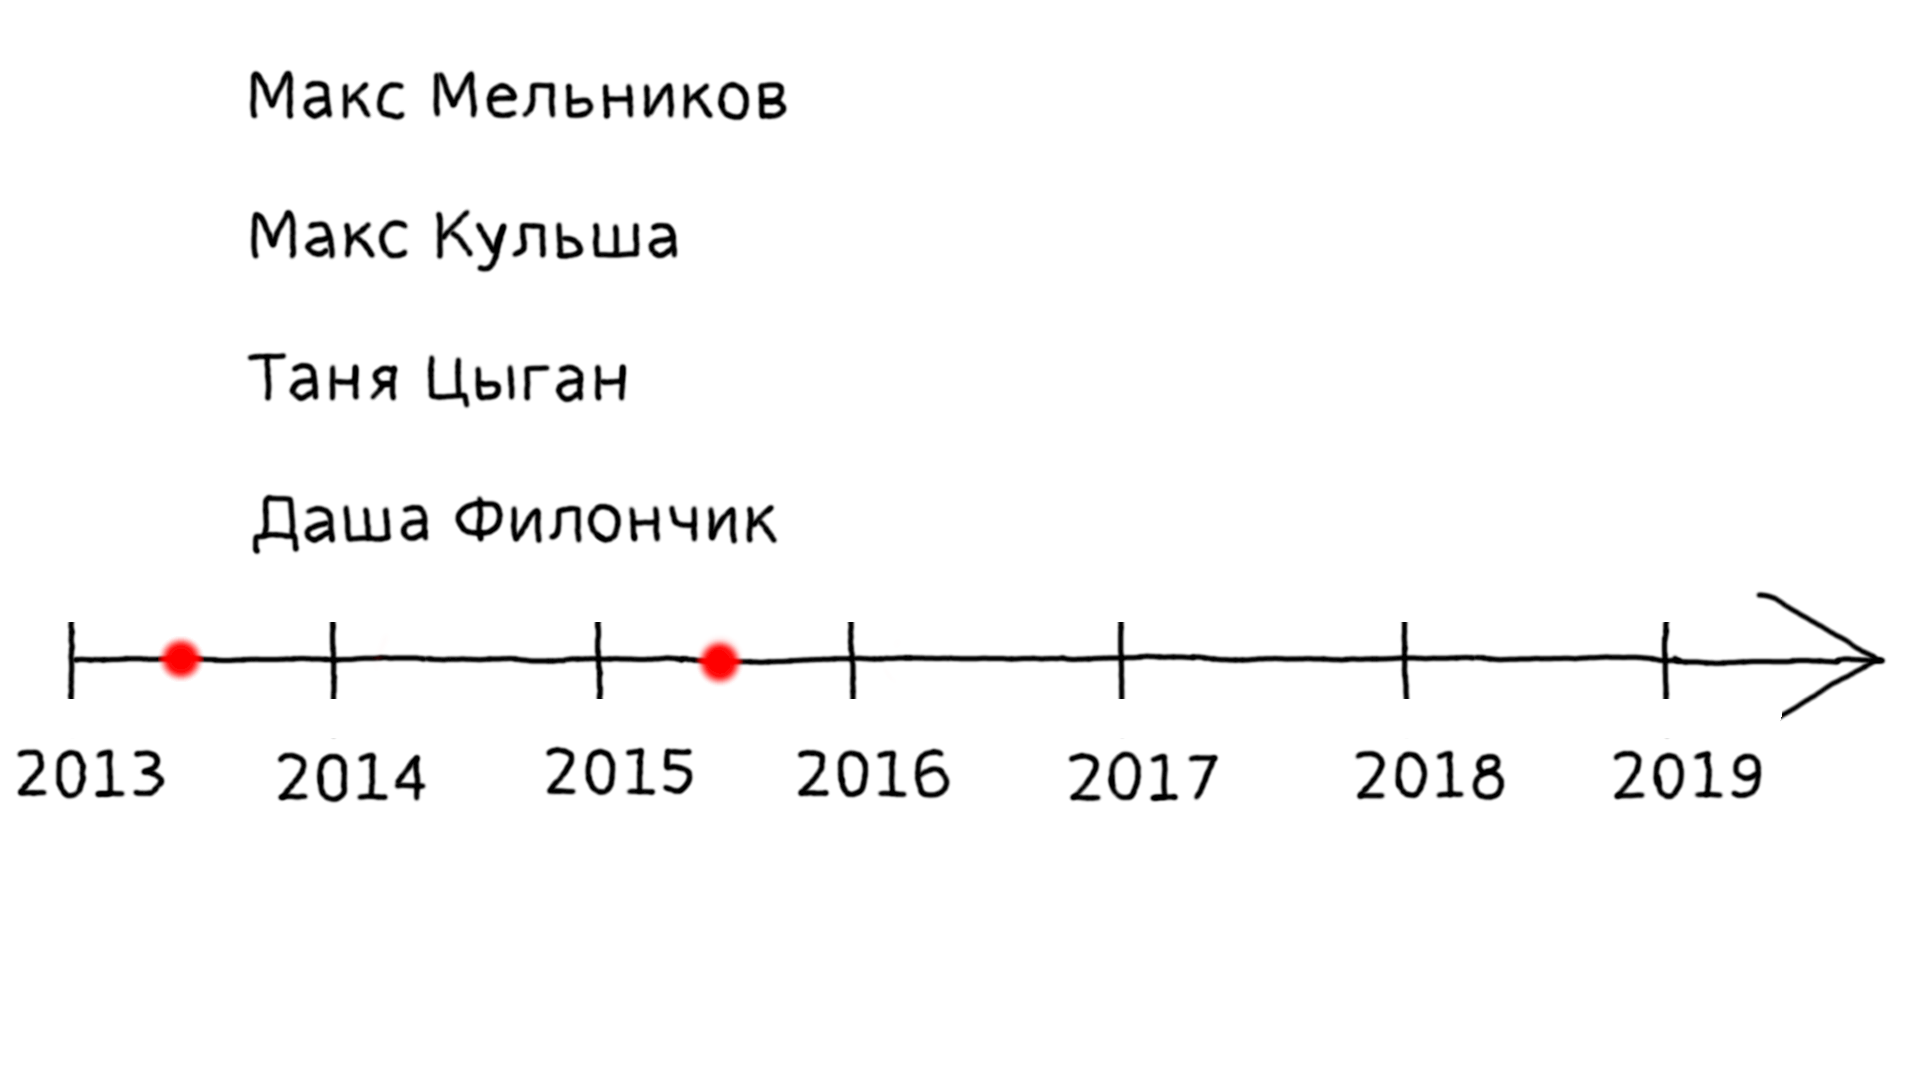
\includegraphics[scale=0.88]{Slides-02-03}
  \end{figure}
\end{frame}

\begin{frame}
  \begin{figure}
    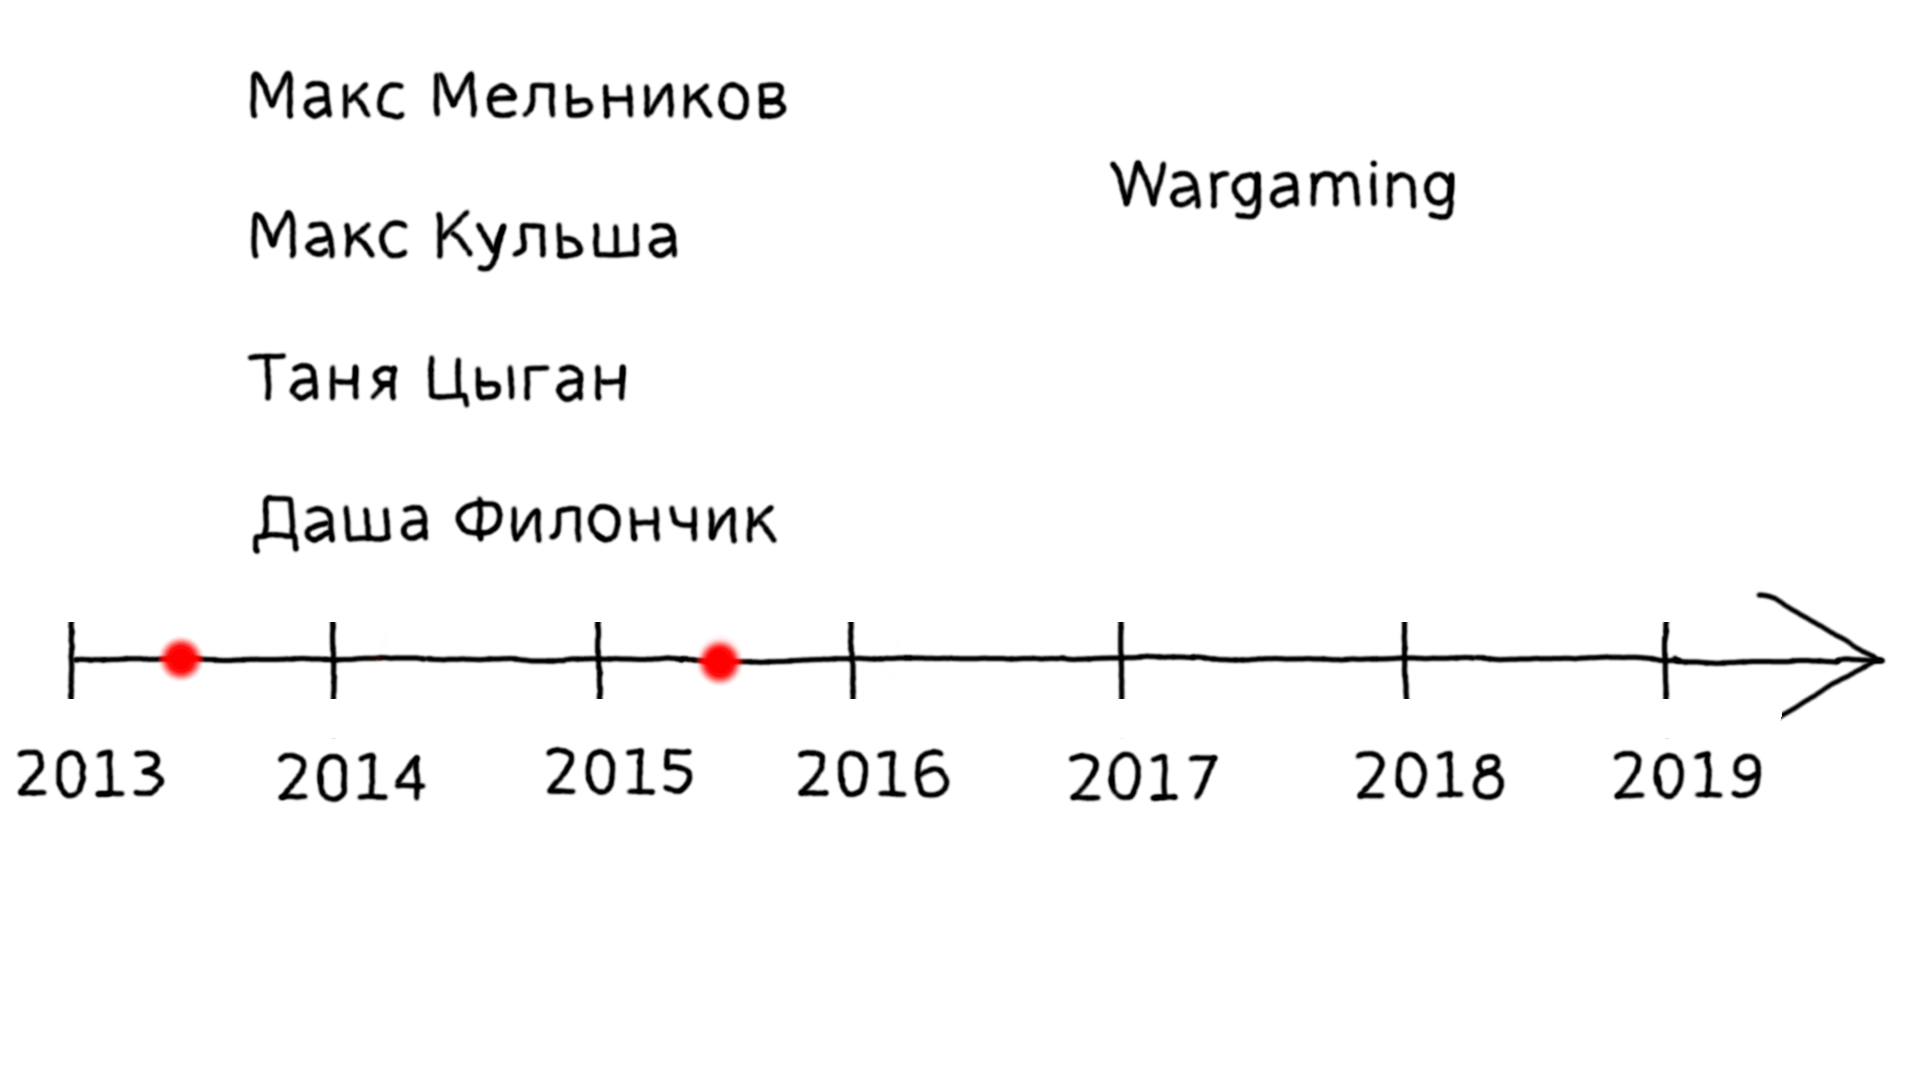
\includegraphics[scale=0.88]{Slides-02-04}
  \end{figure}
\end{frame}

\begin{frame}
  \begin{figure}
    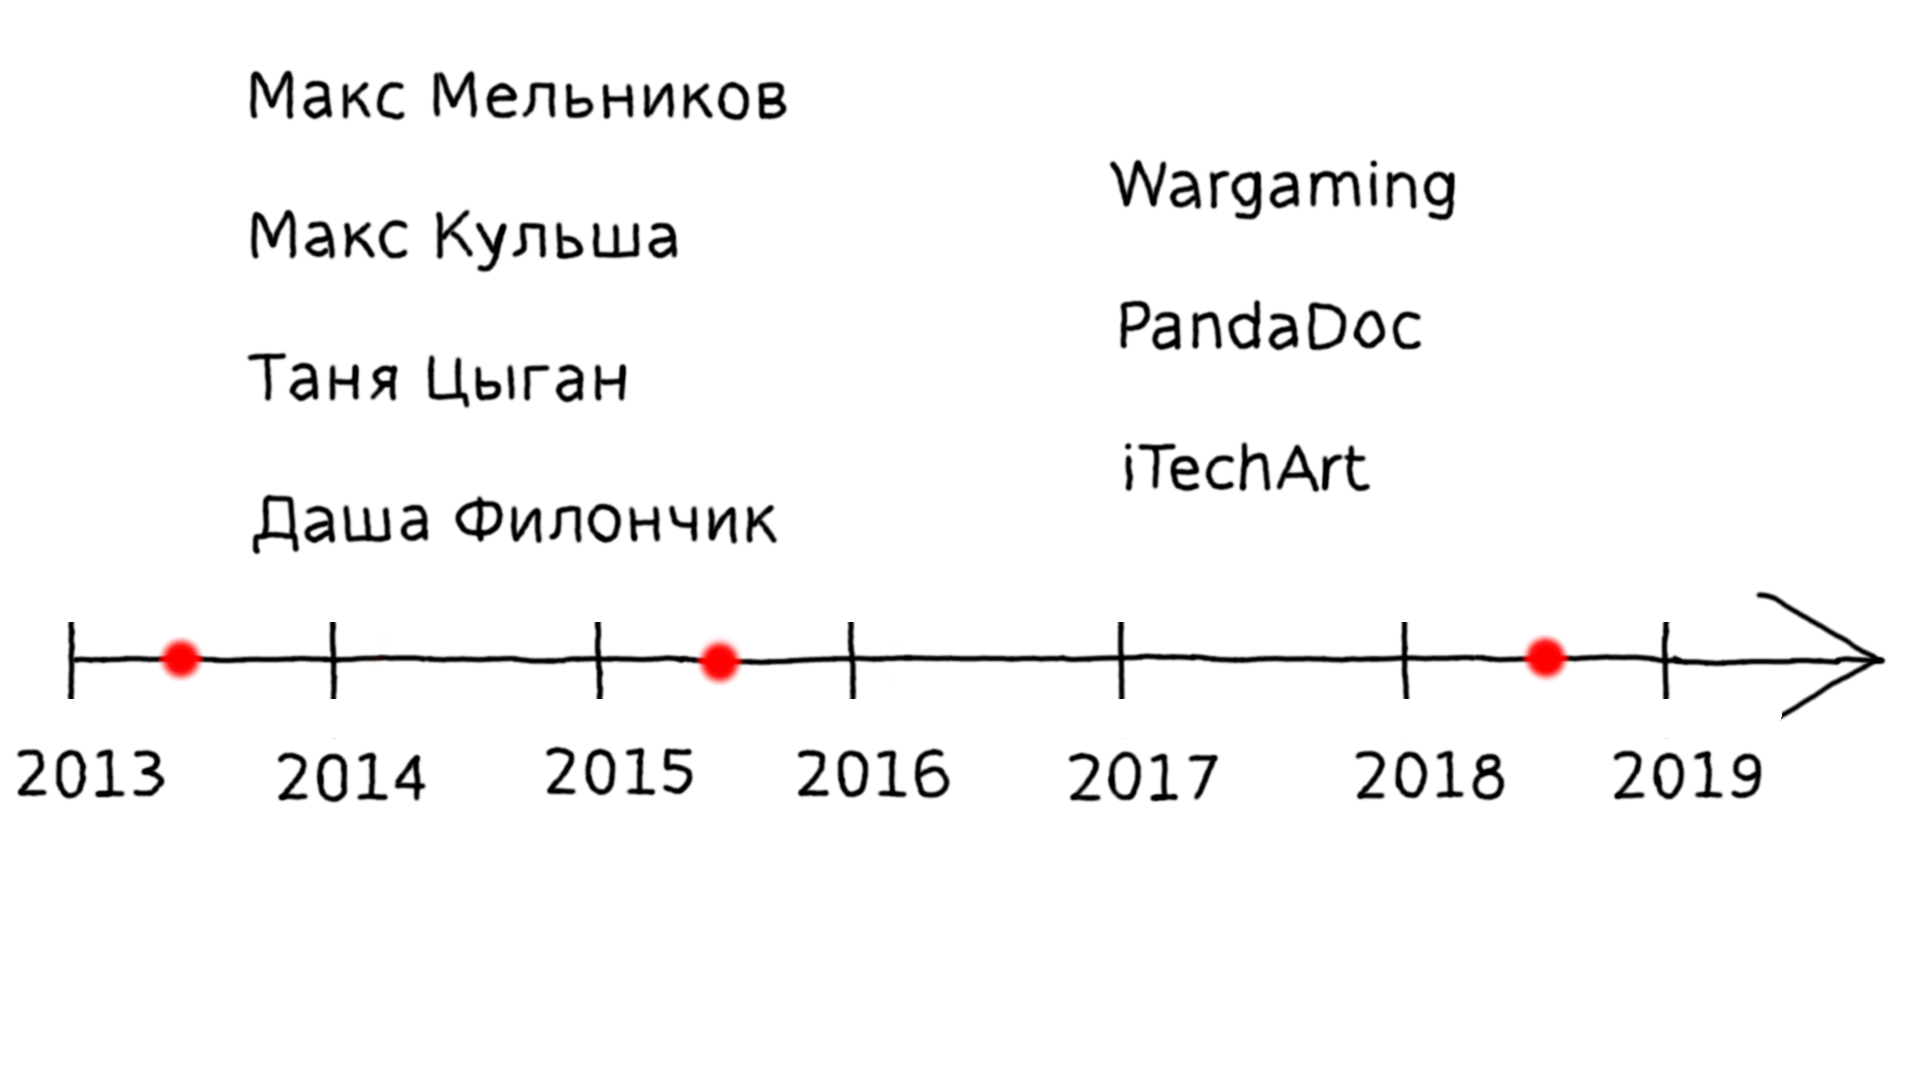
\includegraphics[scale=0.88]{Slides-02-05}
  \end{figure}
\end{frame}

\begin{frame}
  \begin{figure}
    
\includegraphics[scale=0.88]{Slides-03-quote}
  \end{figure}
\end{frame}

\begin{frame}
  \begin{figure}
    
\includegraphics[scale=0.88]{Slides-04-needed}
  \end{figure}
\end{frame}

\begin{frame}
  \begin{figure}
    
\includegraphics[scale=0.88]{Slides-05-help}
  \end{figure}
\end{frame}

\begin{frame}
  \begin{figure}
    
\includegraphics[scale=0.88]{Slides-06-contacts}
  \end{figure}
\end{frame}

\end{document}
